\documentclass[11pt]{article}
\usepackage[margin=1in]{geometry}
\usepackage{amsmath,amssymb,graphicx}
\setlength{\parindent}{0pt}
\setlength{\parskip}{0.45em}
\newcommand{\Rzero}{\mathcal R_0}
\newcommand{\yBL}{y_{\mathrm{BL}}}
\newcommand{\ystar}{y^*}

\begin{document}
\begin{center}
{\Large\bfseries Boundary-layer choice in the generalized epidemic burnout model}
\end{center}
\vspace{0.6em}

\section{The issue}

For
\begin{equation}
 \frac{dx}{d\sigma}=\rho(1-x)x^\theta-\Rzero xy,
 \qquad
 \frac{dy}{d\sigma}=(\Rzero x-1)y,
\end{equation}
the deterministic epidemic tail is matched to the stochastic calculation at
$y=\yBL$. The endemic infectious fraction is
\begin{equation}
 \ystar=\rho(\Rzero-1)\Rzero^{-(1+\theta)}.
\end{equation}
A useful matching line should satisfy
\begin{equation}
 \frac{1}{K}\ll\yBL\ll\rho.
\end{equation}
The first inequality gives many infectives at entry; the second keeps the match
inside the low-prevalence corner regime.

If the line is too low, the deterministic first trough may not reach it, so the
present matching construction has no entry
point. Raising the line increases the region with a usable crossing and may
reduce finite-$K$ entry noise, but may also reduce the accuracy of the local
approximation. The absence of a deterministic
crossing does not imply that the probability of burnout during the first trough
is negligible.

The existing calculations compare
\begin{equation}
 \sqrt{\frac{\ystar}{K}},\qquad
 K^{-1/3}(\ystar)^{2/3},\qquad
 K^{-1/4}(\ystar)^{3/4},\qquad
 \ystar.
\end{equation}
The middle two are the $2/3$ and $3/4$ compromises; $\yBL=\ystar$ is the
highest choice.

\section{What the existing stochastic comparisons show}

Figures~\ref{fig:smallK} and~\ref{fig:largeK} compare unconditional persistence
for the four heights in the finite- and large-$K$ scans. Figure~\ref{fig:conditional}
shows persistence conditional on escaping early fizzle.

\begin{figure}[p]
\centering
\begin{minipage}{0.49\textwidth}\centering
\includegraphics[page=7,trim=15 360 365 70,clip,width=\linewidth]
 {validation/figures/fig09/P1_unconditional_sqrt.pdf}\\
\footnotesize (a) $\yBL=\sqrt{\ystar/K}$
\end{minipage}\hfill
\begin{minipage}{0.49\textwidth}\centering
\includegraphics[page=7,trim=15 360 365 70,clip,width=\linewidth]
 {validation/figures/fig09/P1_unconditional_2_3_compromise.pdf}\\
\footnotesize (b) $2/3$ compromise
\end{minipage}

\vspace{0.7em}
\begin{minipage}{0.49\textwidth}\centering
\includegraphics[page=7,trim=15 360 365 70,clip,width=\linewidth]
 {validation/figures/fig09/P1_unconditional_3_4_compromise.pdf}\\
\footnotesize (c) $3/4$ compromise
\end{minipage}\hfill
\begin{minipage}{0.49\textwidth}\centering
\includegraphics[page=7,trim=15 360 365 70,clip,width=\linewidth]
 {validation/figures/fig09/P1_unconditional_ystar.pdf}\\
\footnotesize (d) $\yBL=\ystar$
\end{minipage}
\caption{Unconditional persistence: Figure 9 subset with $\rho=0.05$,
$\theta=0$, $K=1000$.}
\label{fig:smallK}
\end{figure}

\begin{figure}[p]
\centering
\begin{minipage}{0.49\textwidth}\centering
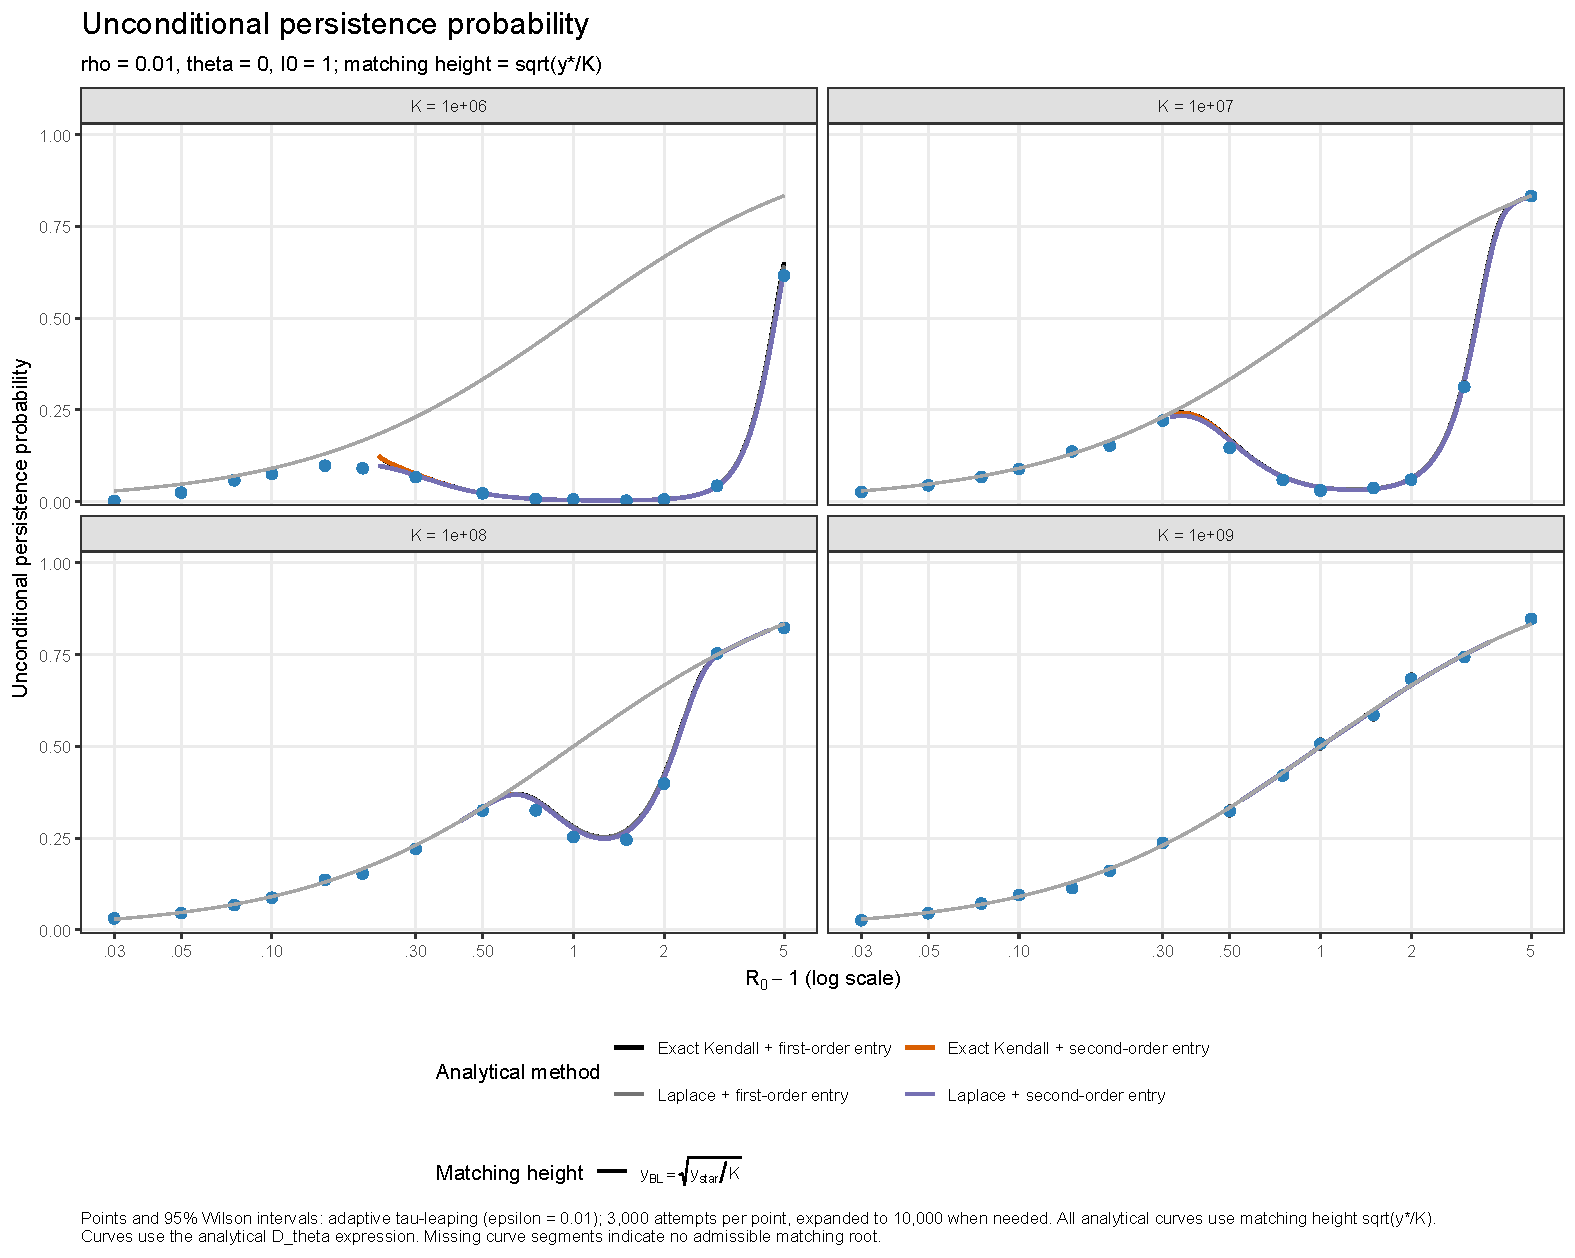
\includegraphics[page=1,trim=15 360 365 70,clip,width=\linewidth]
 {validation/figures/fig11/P1_stochastic_validation_sqrt.pdf}\\
\footnotesize (a) $\yBL=\sqrt{\ystar/K}$
\end{minipage}\hfill
\begin{minipage}{0.49\textwidth}\centering
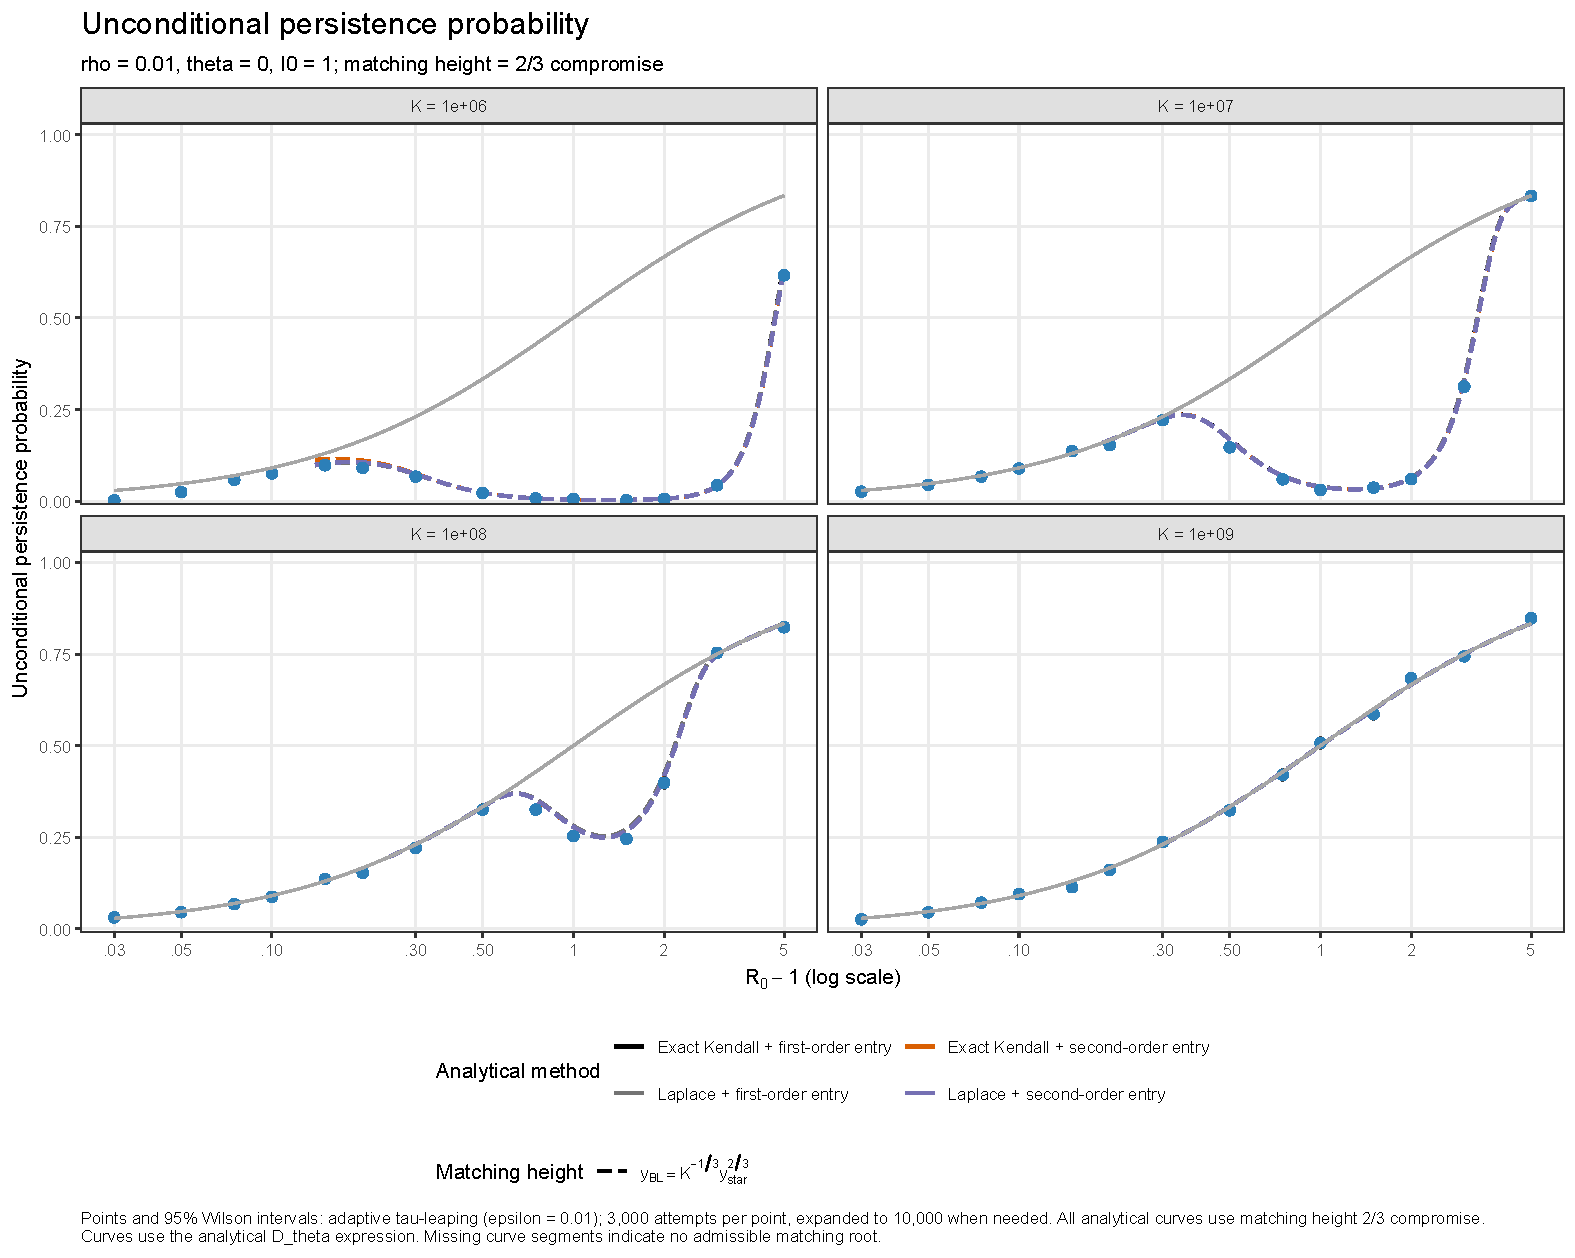
\includegraphics[page=1,trim=15 360 365 70,clip,width=\linewidth]
 {validation/figures/fig11/P1_stochastic_validation_2_3_compromise.pdf}\\
\footnotesize (b) $2/3$ compromise
\end{minipage}

\vspace{0.7em}
\begin{minipage}{0.49\textwidth}\centering
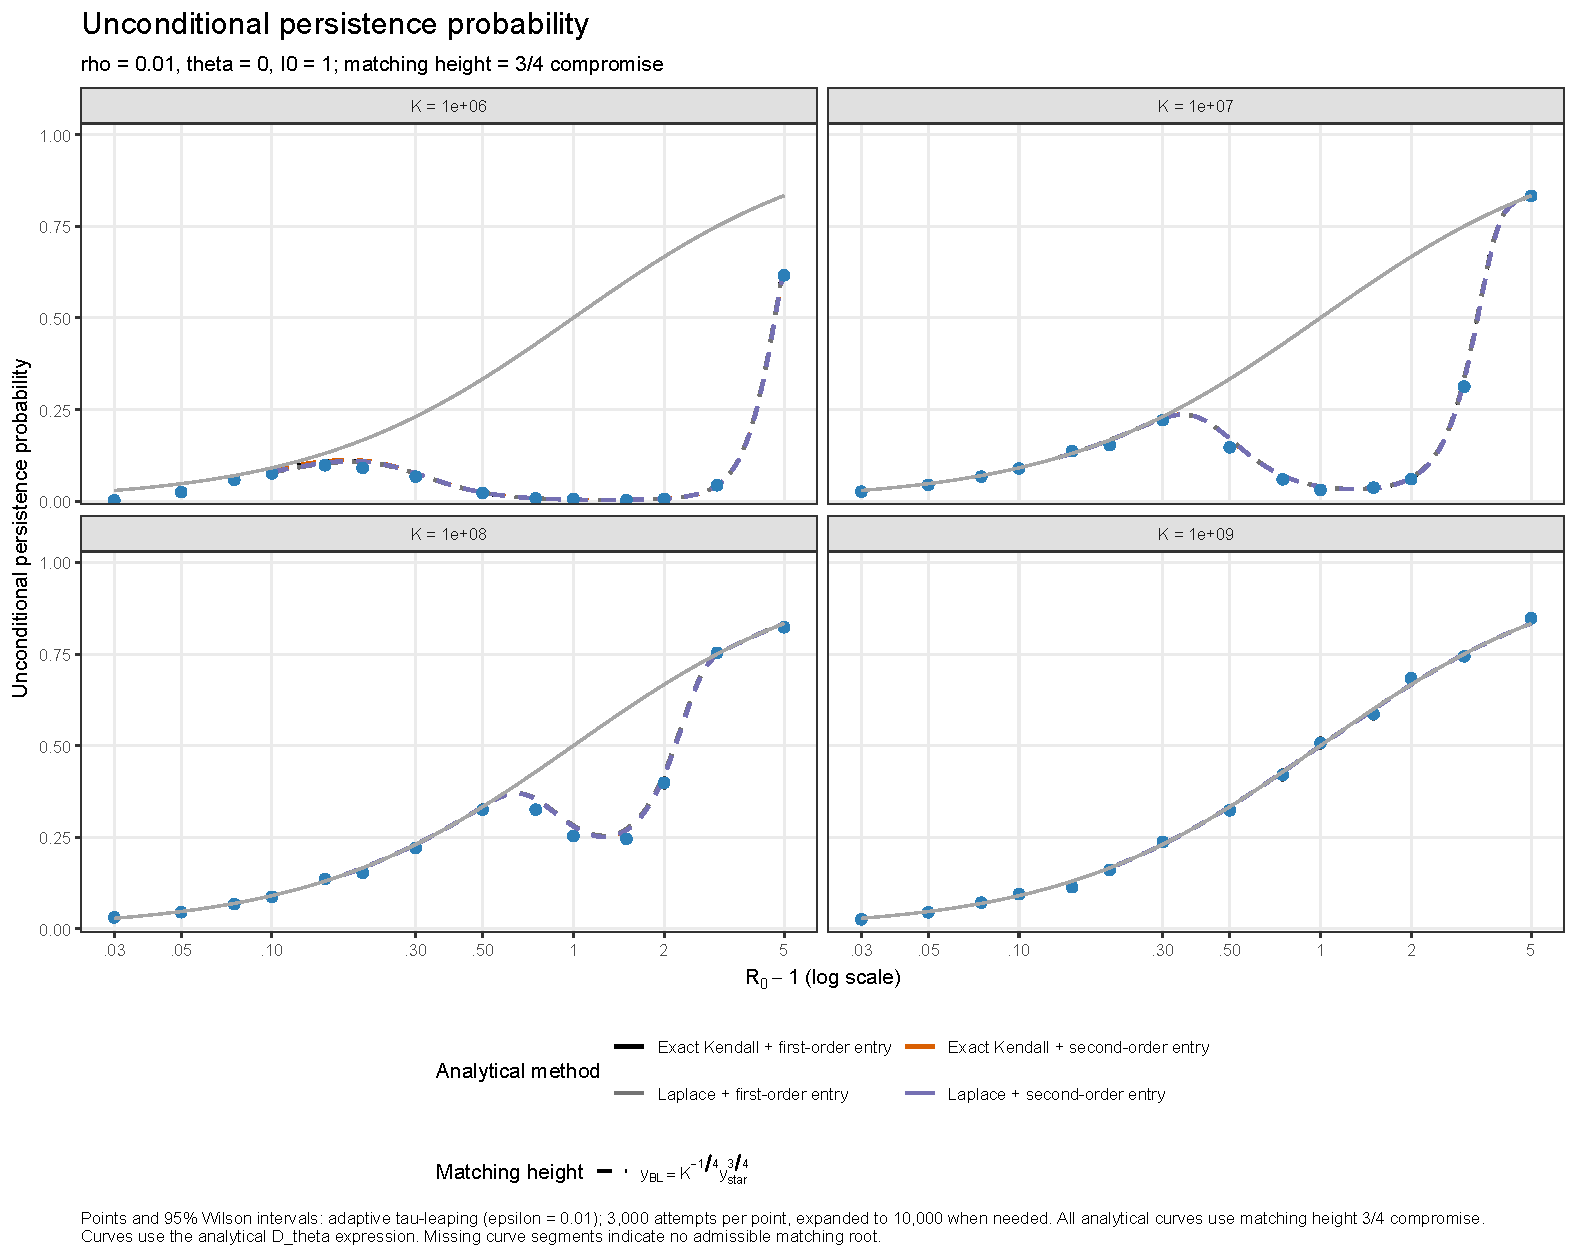
\includegraphics[page=1,trim=15 360 365 70,clip,width=\linewidth]
 {validation/figures/fig11/P1_stochastic_validation_3_4_compromise.pdf}\\
\footnotesize (c) $3/4$ compromise
\end{minipage}\hfill
\begin{minipage}{0.49\textwidth}\centering
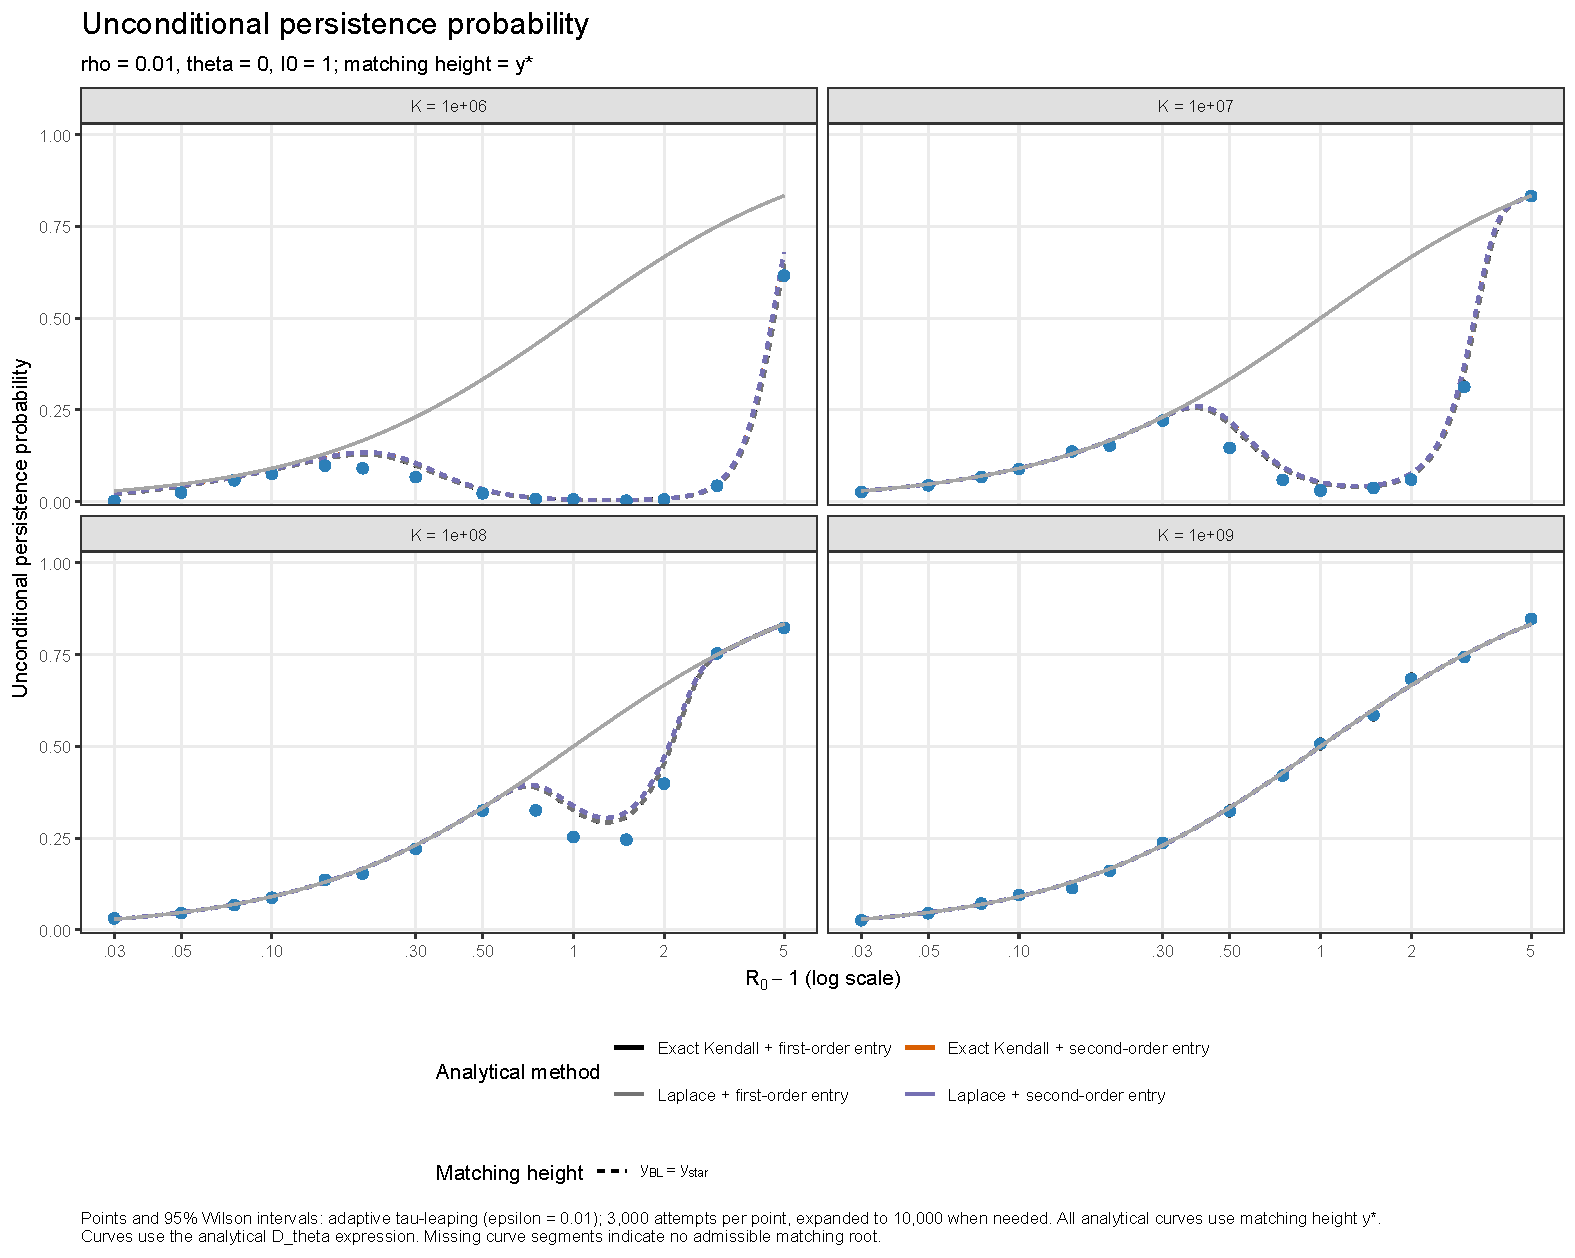
\includegraphics[page=1,trim=15 360 365 70,clip,width=\linewidth]
 {validation/figures/fig11/P1_stochastic_validation_ystar.pdf}\\
\footnotesize (d) $\yBL=\ystar$
\end{minipage}
\caption{Unconditional persistence: Figure 11 subset with $\rho=0.01$,
$\theta=0$, $K=10^6$.}
\label{fig:largeK}
\end{figure}

\begin{figure}[p]
\centering
\begin{minipage}{0.49\textwidth}\centering
\includegraphics[page=7,trim=15 360 365 70,clip,width=\linewidth]
 {validation/figures/fig10/P1_conditional_sqrt.pdf}\\
\footnotesize (a) $\yBL=\sqrt{\ystar/K}$
\end{minipage}\hfill
\begin{minipage}{0.49\textwidth}\centering
\includegraphics[page=7,trim=15 360 365 70,clip,width=\linewidth]
 {validation/figures/fig10/P1_conditional_2_3_compromise.pdf}\\
\footnotesize (b) $2/3$ compromise
\end{minipage}

\vspace{0.7em}
\begin{minipage}{0.49\textwidth}\centering
\includegraphics[page=7,trim=15 360 365 70,clip,width=\linewidth]
 {validation/figures/fig10/P1_conditional_3_4_compromise.pdf}\\
\footnotesize (c) $3/4$ compromise
\end{minipage}\hfill
\begin{minipage}{0.49\textwidth}\centering
\includegraphics[page=7,trim=15 360 365 70,clip,width=\linewidth]
 {validation/figures/fig10/P1_conditional_ystar.pdf}\\
\footnotesize (d) $\yBL=\ystar$
\end{minipage}
\caption{Persistence conditional on escaping early fizzle: Figure 10 subset
with $\rho=0.05$, $\theta=0$, $K=1000$.}
\label{fig:conditional}
\end{figure}

\end{document}
